\documentclass[conf]{new-aiaa}

\usepackage{float}
\usepackage{subfigure}
\usepackage[justification=centering]{caption}
\usepackage{multirow} \usepackage{graphicx}
\graphicspath{ {./images/} }
\usepackage{nameref}
\usepackage{amsmath}
\usepackage{amssymb}
\usepackage{amsfonts}
\usepackage[linesnumbered,ruled]{algorithm2e}
\usepackage{tikz}
\usetikzlibrary{calc,patterns,decorations.pathmorphing,decorations.markings,positioning,automata,shapes,arrows}
\tikzstyle{block} = [rectangle, draw, text width=3.5cm]
\tikzstyle{line} = [draw, -latex']
\usepackage{pgfplots}
\usepgfplotslibrary{colormaps,external}
\usepackage{ulem}
\usepackage{verbatim}
\usepackage[version=4]{mhchem}
\usepackage{siunitx}
\usepackage{pbox}
\usepackage{longtable,tabularx}
\setlength\LTleft{0pt} 

\title{ Deformation Modeled with  Creep and Multiplicatively-Decomposed Plasticity
        of a Panel in High Speed Flow}
      

\author{Justin L. Clough%
        \footnote{
          PhD Student, 
          justin.clough1@gmail.com,
          Aerospace and Mechanical Engineering Department, 
          854 Downey Way, RRB 101.}
        and Assad A. Oberai%
        \footnote{  
          Professor, 
          Aerospace and Mechanical Engineering Department, 
          854 Downey Way, RRB 101.}}
\affil{University of Southern California,
       Los Angeles, CA, 90089}
\begin{document}
\maketitle

\begin{abstract}
abstract text
\end{abstract}

\section{Nomenclature}

{\renewcommand\arraystretch{1.0}
\noindent\begin{longtable*}{@{}l @{\quad=\quad} l@{}}
Ma & Mach number
\end{longtable*}}

\section{Introduction}
% Outline:
% - Overview of hypersonic structures
% - What is high speed flow? Characteristics
% - When does and doesn't inertia matter?
% - When does large strain matter?
% - What is creep/ Norton creep?

The skin of a high speed vehicle must support both
the aerodynamic tractions and heating during flight;
it is typically designed as a thin face plate supported 
by stiffeners 
\cite{
  mcnamara_aeroelastic_and_aerothermoelastic_analysis_in_hypersonic_flow_past_present_and_future, 
  riley_interaction_between_aerothermally_compliant_structures_and_boudnary_layer_transition_in_hypersonic_flow,
  spottswood_exploring_the_response_of_a_thin_flexible_panel,
  thornton_coupled_flow_thermal_and_structural_analysis_of_aerodynamically_heated_panels,
  savino_aerothermodynamic_study_of_ultrahigh_termperature_cermaic_winglet_for_atmospheric_reentry_test}.
Some examples of typical panel stiffener geometries are
shown in Figure \ref{fig_example_stiffener_geoms} from 
\cite{
  zuchowski_AVIATR_Predictive_capability_for_hypersonic_structural_response_and_life_prediction_phase_II}.

\begin{figure}[H] 
  \centering
    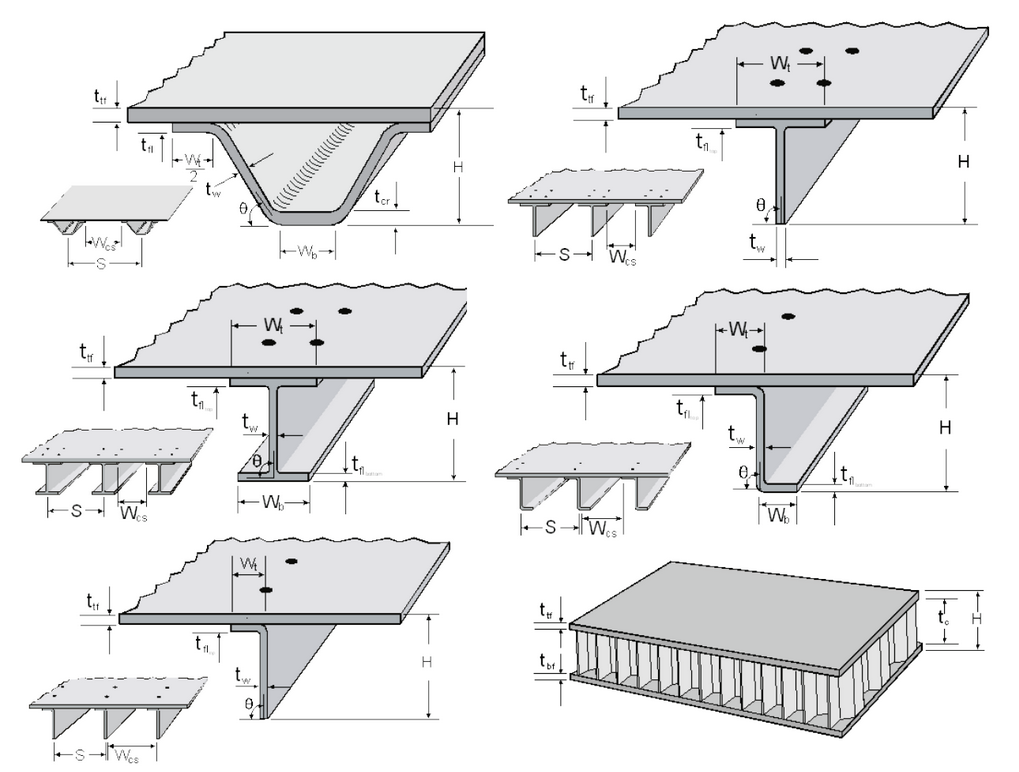
\includegraphics[width=0.95\textwidth, keepaspectratio]
    {example_stiffener_geoms}
  \caption{ 
          Geometry of stiffener options of typical panels for high speed vehicles.
            Adapted from \cite{
  zuchowski_AVIATR_Predictive_capability_for_hypersonic_structural_response_and_life_prediction_phase_II}.
          }
  \label{fig_example_stiffener_geoms}
\end{figure}

High speed flow over a vehicle creates a harsh environment.
For example, the skin of the X-15 regularly saw temperatures
as high as 1220$^{\circ}$ F
during its flights up to 6.7 Ma.
\cite{ kordes_structureal_heating_experiencs_on_the_x15_airplane}.


Note to the reviewers: A more extensive review of the 
state of the art will be included in the 
final manuscript.

\section{Methods} \label{sec_methods}
% outline:
%  - Panel geometry
%  - Multi materials -> Ti6242, Al 7075 (like McNamara)
%  - Creep + Plasticity
%  - Loading? Historical temperature?
The goal of this study is to model the large creep deformation a canonical acreage
panel due to the thermal loads experience from a high speed flight.



The geometry of the panel considered for this study is borrowed from
\cite{ 
  plews_a_two_scale_generalized_finite_element_approach_for_modeling_localized_thermoplasticity}.
An image of this is shown in Figure \ref{fig_plews_panel_geom}.

\begin{figure}[H] 
  \centering
    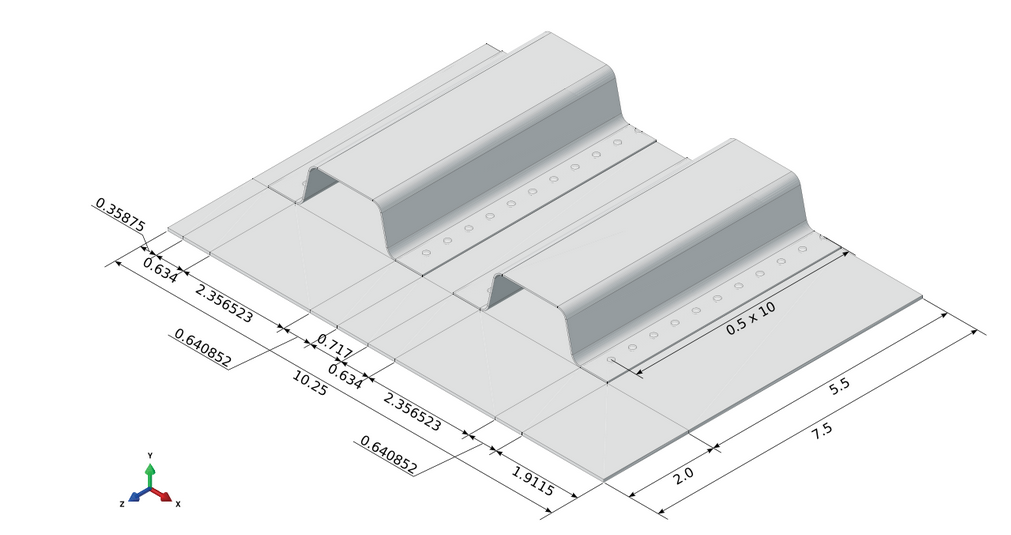
\includegraphics[width=0.95\textwidth, keepaspectratio]
    {plews_panel_geom}
  \caption{ Geometry of the acreage panel of interest. 
            All dimensions in inches.
            Adapted from \cite{
    plews_a_two_scale_generalized_finite_element_approach_for_modeling_localized_thermoplasticity}.
          }
  \label{fig_plews_panel_geom}
\end{figure}

% \section{Discussion and Closing Remarks} \label{sec_closing_remarks}
% discussion text

% \section{Future Work} \label{sec_future}
% future work text
% 
% \section*{Acknowledgments}
% The authors thank the DoD Science, Mathematics, And 
% Research for Transformation (SMART) Scholarship
% for Service Program which sponsored this work.

\bibliography{monolith.bib}

\end{document}
